\documentclass[12pt,t,aspectratio=169]{beamer}
\usepackage{graphicx}
\setbeameroption{hide notes}
\setbeamertemplate{note page}[plain]
\usepackage{listings}

% header.tex: boring LaTeX/Beamer details + macros

% get rid of junk
\usetheme{default}
\beamertemplatenavigationsymbolsempty
\hypersetup{pdfpagemode=UseNone} % don't show bookmarks on initial view


% font
\usepackage{fontspec}
\setsansfont
  [ ExternalLocation = fonts/ ,
    UprightFont = *-regular ,
    BoldFont = *-bold ,
    ItalicFont = *-italic ,
    BoldItalicFont = *-bolditalic ]{texgyreheros}
\setbeamerfont{note page}{family*=pplx,size=\footnotesize} % Palatino for notes
% "TeX Gyre Heros can be used as a replacement for Helvetica"
% I've placed them in fonts/; alternatively you can install them
% permanently on your system as follows:
%     Download http://www.gust.org.pl/projects/e-foundry/tex-gyre/heros/qhv2.004otf.zip
%     In Unix, unzip it into ~/.fonts
%     In Mac, unzip it, double-click the .otf files, and install using "FontBook"

% named colors
\definecolor{offwhite}{RGB}{255,250,240}
\definecolor{gray}{RGB}{155,155,155}

% USE LIGHT BACKGROUND HERE
%\ifx\notescolors\undefined % slides
%  \definecolor{foreground}{RGB}{255,255,255}
%  \definecolor{background}{RGB}{24,24,24}
%  \definecolor{title}{RGB}{107,174,214}
%  \definecolor{subtitle}{RGB}{128,128,214}
%  \definecolor{hilit}{RGB}{102,255,204}
%  \definecolor{vhilit}{RGB}{255,111,207}
%  \definecolor{lolit}{RGB}{155,155,155}
%  \definecolor{myyellow}{rgb}{1,1,0.7}
%\else % notes
  \definecolor{background}{RGB}{255,255,255}
  \definecolor{foreground}{RGB}{24,24,24}
  \definecolor{title}{RGB}{27,94,134}
  \definecolor{subtitle}{RGB}{22,175,124}
  \definecolor{hilit}{RGB}{122,0,128}
  \definecolor{vhilit}{RGB}{255,0,128}
  \definecolor{lolit}{RGB}{95,95,95}
%\fi
\definecolor{nhilit}{RGB}{128,0,128}  % hilit color in notes
\definecolor{nvhilit}{RGB}{255,0,128} % vhilit for notes

\newcommand{\hilit}{\color{hilit}}
\newcommand{\vhilit}{\color{vhilit}}
\newcommand{\nhilit}{\color{nhilit}}
\newcommand{\nvhilit}{\color{nvhilit}}
\newcommand{\lolit}{\color{lolit}}

% use those colors
\setbeamercolor{titlelike}{fg=title}
\setbeamercolor{subtitle}{fg=subtitle}
\setbeamercolor{institute}{fg=lolit}
\setbeamercolor{normal text}{fg=foreground,bg=background}
\setbeamercolor{item}{fg=foreground} % color of bullets
\setbeamercolor{subitem}{fg=lolit}
\setbeamercolor{itemize/enumerate subbody}{fg=lolit}
\setbeamertemplate{itemize subitem}{{\textendash}}
\setbeamerfont{itemize/enumerate subbody}{size=\footnotesize}
\setbeamerfont{itemize/enumerate subitem}{size=\footnotesize}

% page number
\setbeamertemplate{footline}{%
    \raisebox{5pt}{\makebox[\paperwidth]{\hfill\makebox[20pt]{\lolit
          \scriptsize\insertframenumber}}}\hspace*{5pt}}

% add a bit of space at the top of the notes page
\addtobeamertemplate{note page}{\setlength{\parskip}{12pt}}

% default link color
\hypersetup{colorlinks, urlcolor={hilit}}

\ifx\notescolors\undefined % slides
  % set up listing environment
  \lstset{language=bash,
          basicstyle=\ttfamily\scriptsize,
          frame=single,
          commentstyle=,
          backgroundcolor=\color{darkgray},
          showspaces=false,
          showstringspaces=false
          }
\else % notes
  \lstset{language=bash,
          basicstyle=\ttfamily\scriptsize,
          frame=single,
          commentstyle=,
          backgroundcolor=\color{offwhite},
          showspaces=false,
          showstringspaces=false
          }
\fi

% a few macros
\newcommand{\bi}{\begin{itemize}}
\newcommand{\bbi}{\vspace{24pt} \begin{itemize} \itemsep8pt}
\newcommand{\ei}{\end{itemize}}
\newcommand{\ig}{\includegraphics}
\newcommand{\subt}[1]{{\footnotesize \color{subtitle} {#1}}}
\newcommand{\ttsm}{\tt \small}
\newcommand{\ttfn}{\tt \footnotesize}
\newcommand{\figh}[2]{\centerline{\includegraphics[height=#2\textheight]{#1}}}
\newcommand{\figw}[2]{\centerline{\includegraphics[width=#2\textwidth]{#1}}}


%%%%%%%%%%%%%%%%%%%%%%%%%%%%%%%%%%%%%%%%%%%%%%%%%%%%%%%%%%%%%%%%%%%%%%
% end of header
%%%%%%%%%%%%%%%%%%%%%%%%%%%%%%%%%%%%%%%%%%%%%%%%%%%%%%%%%%%%%%%%%%%%%%

% title info
\title{Opportunities in \\ biomedical data science}
\subtitle{}
\author{\href{https://kbroman.org}{Karl Broman}}
\institute{Biostatistics \& Medical Informatics, UW{\textendash}Madison}
\date{\href{https://kbroman.org}{\tt \scriptsize \color{foreground} kbroman.org}
\\[-4pt]
\href{https://github.com/kbroman}{\tt \scriptsize \color{foreground} github.com/kbroman}
\\[-4pt]
\href{https://twitter.com/kwbroman}{\tt \scriptsize \color{foreground} @kwbroman}
\\[2pt]
\scriptsize {\lolit Slides:} \href{https://bit.ly/carleton2019}{\tt \scriptsize
  \color{foreground} bit.ly/carleton2019}
}


\begin{document}

% title slide
{
\setbeamertemplate{footline}{} % no page number here
\frame{
  \titlepage



  \note{These are slides for a short, informal talk that I will gave at
    Carleton College on 1 Oct 2019

    Source: {\tt https://github.com/kbroman/Talk\_Carleton2019} \\
    Slides: {\tt https://bit.ly/carleton2019}
}
} }



\begin{frame}{Biomedical data explosion}

  \bbi
\item Electronic health records (EHR)

\item Imaging

\item Genome/proteome/metabolome/microbiome data

\item Personal activity/health tracking devices

  \only<2>{
    \item High-throughput measurements in agriculture and ecology
  }

  \ei

\end{frame}


\begin{frame}[c]{}

\centerline{
  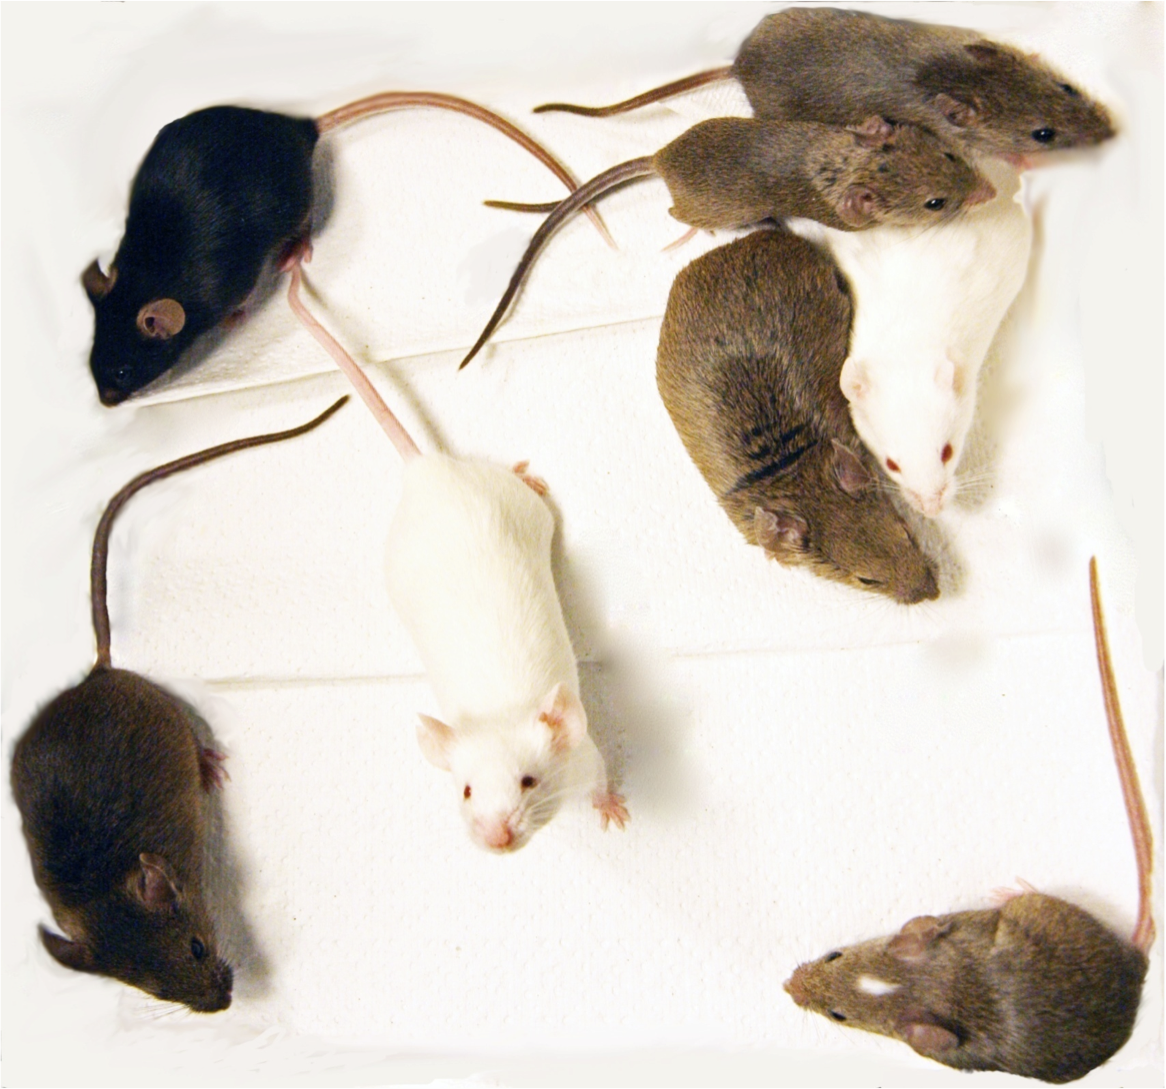
\includegraphics[height=1.05\textheight]{Figs/cc_founders.png}
}

\end{frame}


\begin{frame}{}

\vspace*{8mm}

\hspace*{6mm}
\centerline{
\begin{minipage}[t]{60mm}
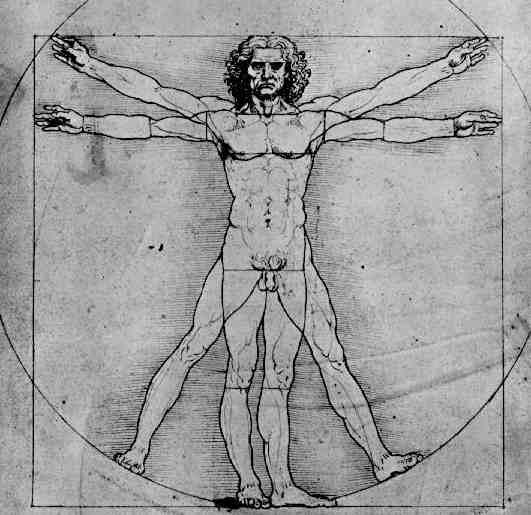
\includegraphics[height=60mm]{Figs/da-vinci-man.jpg}
\end{minipage}
\hspace{15mm}
\begin{minipage}[t]{60mm}
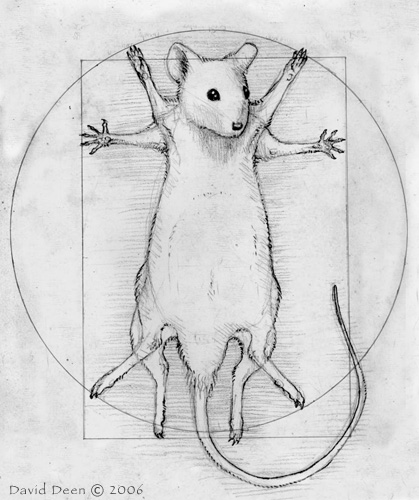
\includegraphics[height=60mm]{Figs/vitruvian_mouse.jpg}
\hspace{5mm}
\href{http://daviddeen.com}{\scriptsize \lolit \tt daviddeen.com}
\end{minipage}
}


\note{
Mice are not humans, but you can learn a great deal about human
biology and disease from mice.

The figure on the right is from David Deen.
}

\end{frame}




\begin{frame}{Intercross}

\centerline{
  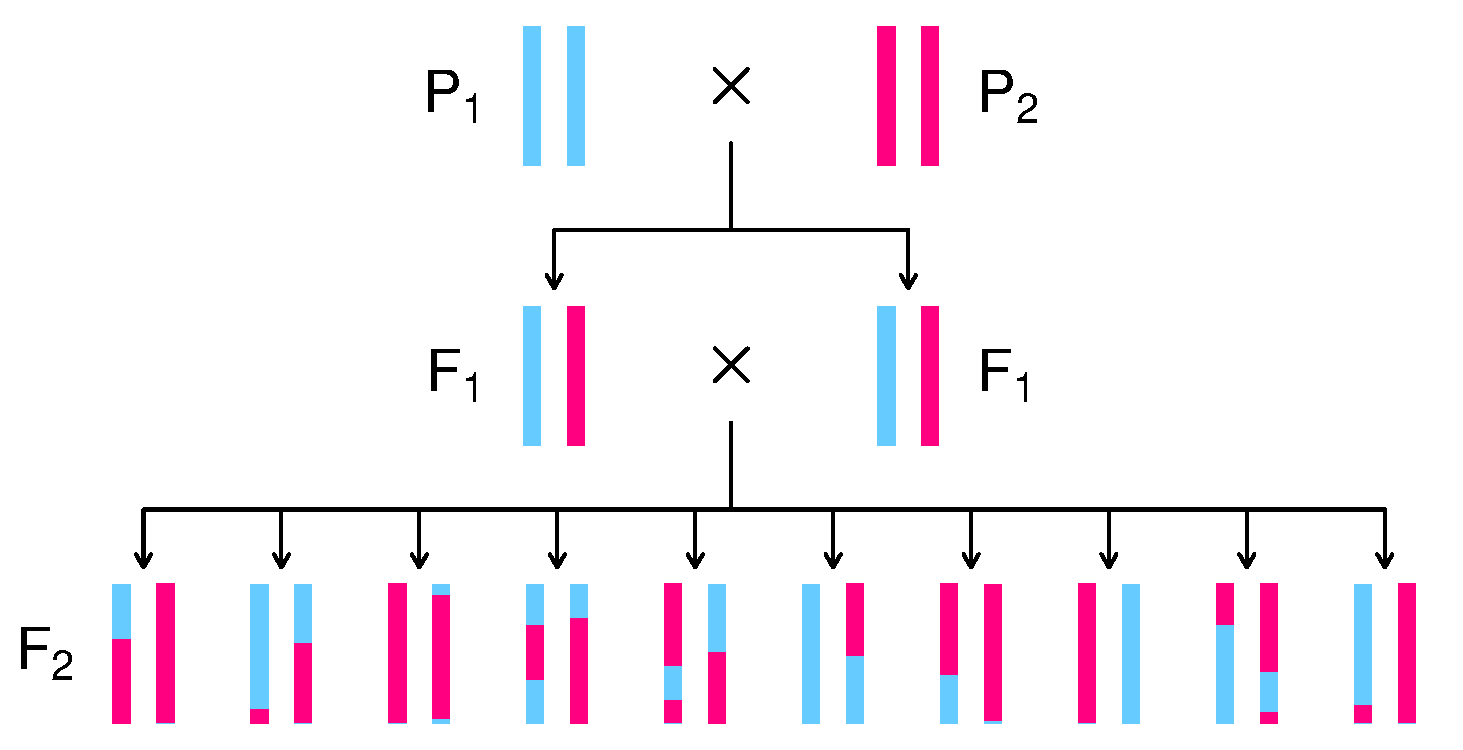
\includegraphics[height=0.9\textheight]{Figs/intercross_light.pdf}
}

\end{frame}


\begin{frame}{Genome scan}

\only<1>{\centerline{
  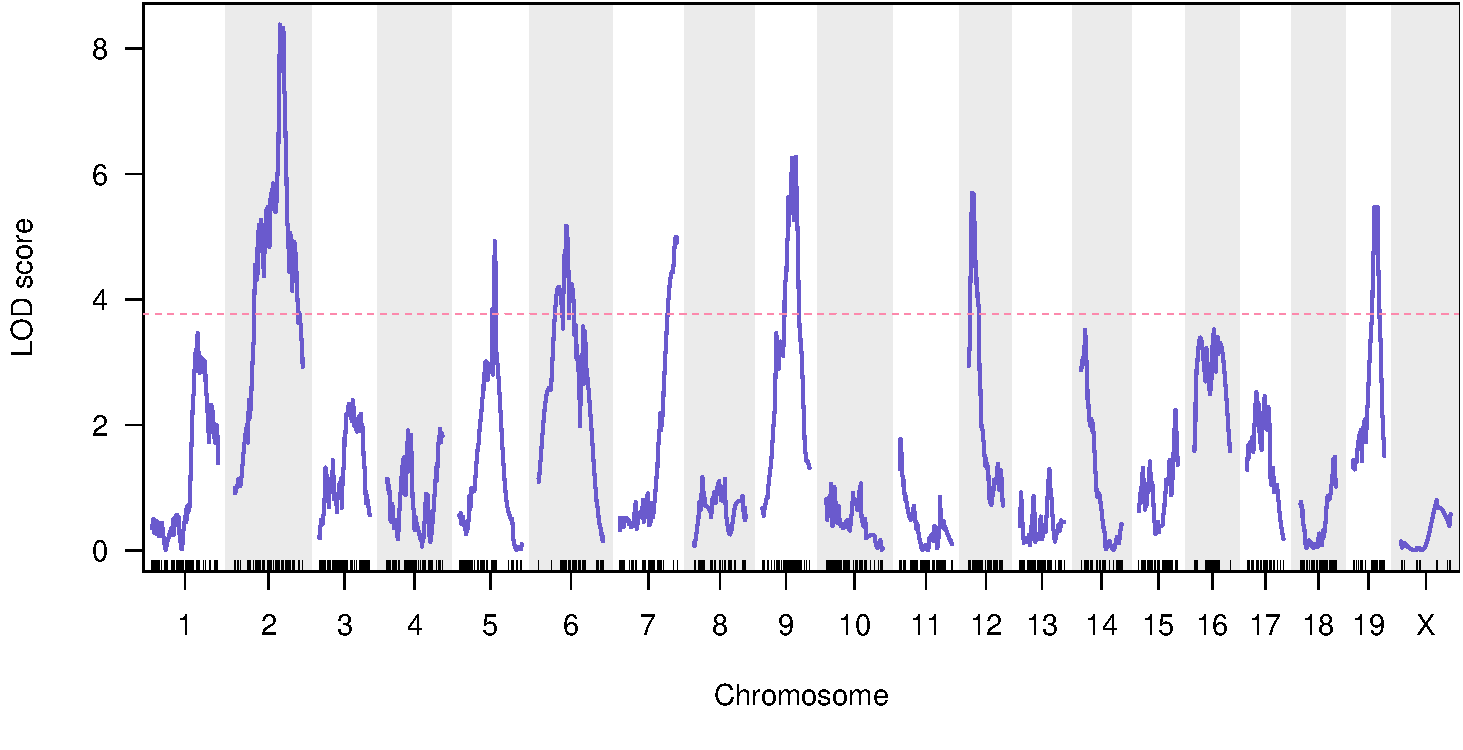
\includegraphics[height=0.93\textheight]{Figs/lodcurve_insulin_light.pdf}
  }}

\only<2>{\centerline{
  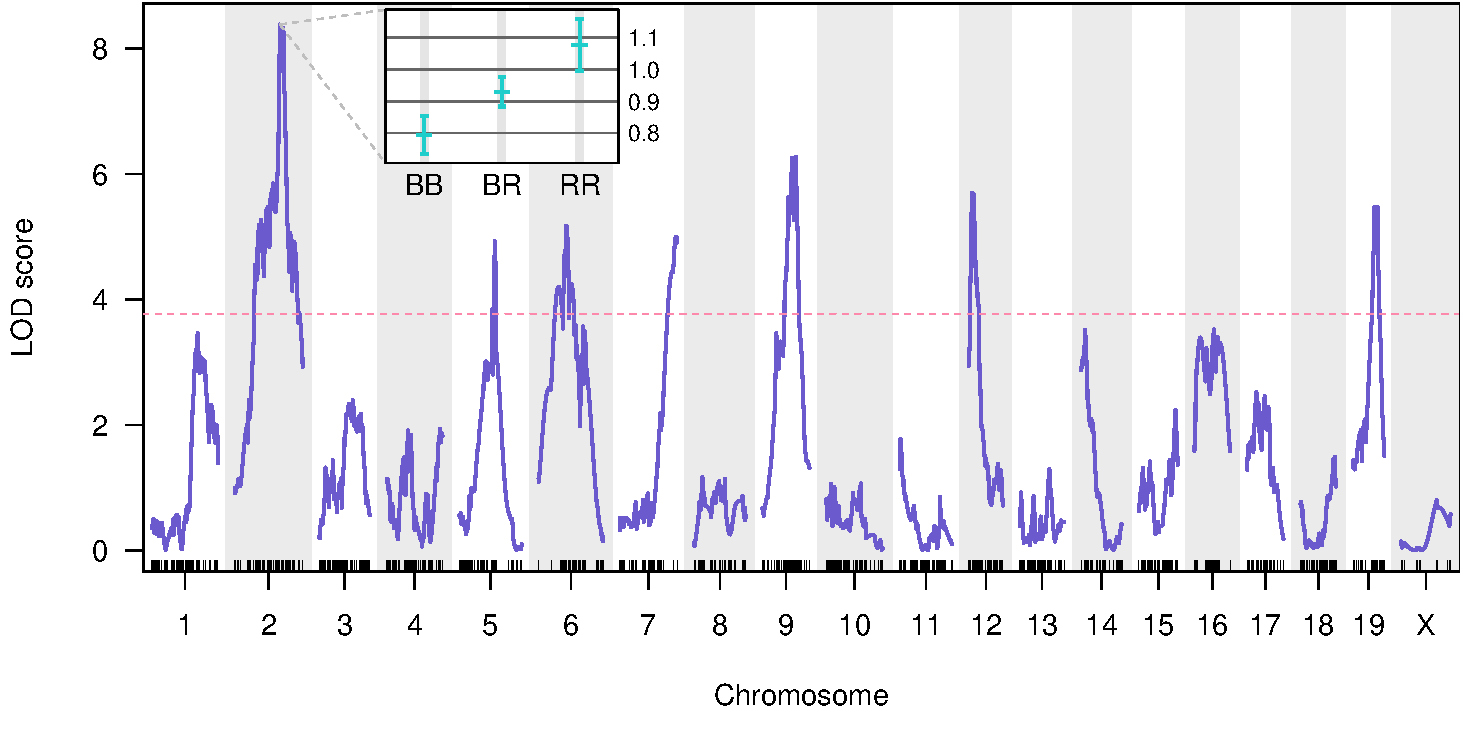
\includegraphics[height=0.93\textheight]{Figs/lodcurve_insulin_with_effects_light.pdf}
  }}

\end{frame}


\begin{frame}{High-throughput phenotypes}

\only<1>{ \centerline{
  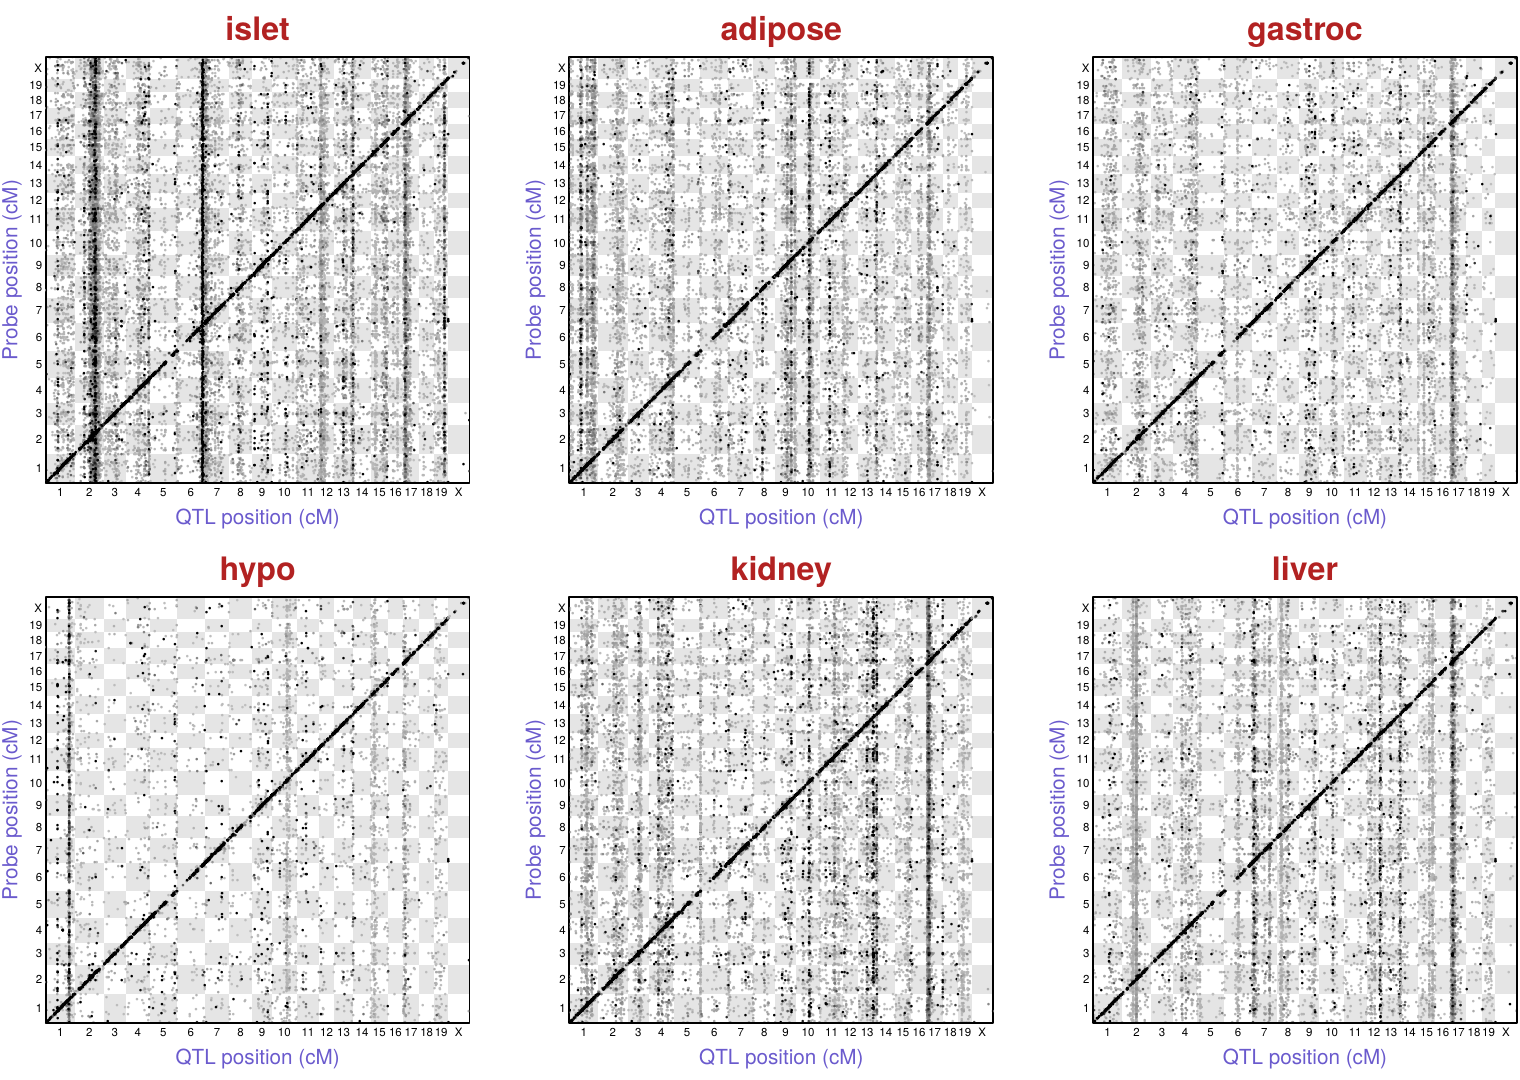
\includegraphics[height=0.92\textheight]{Figs/eqtl_cistrans.png}
    } }

\only<2>{ \centerline{
  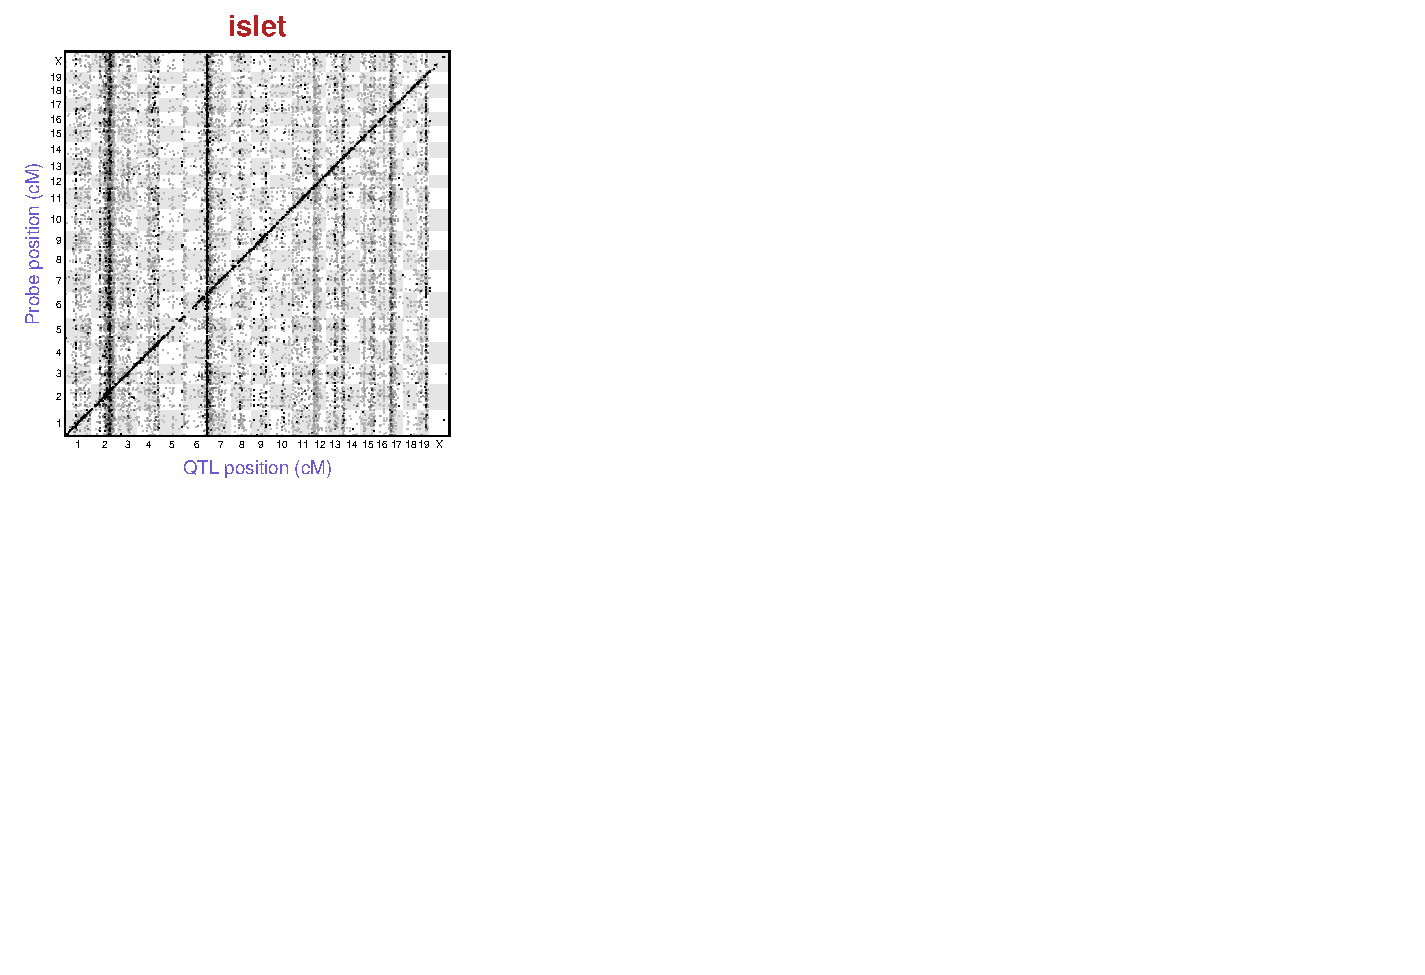
\includegraphics[height=0.93\textheight]{Figs/eqtl_cistrans_islet.pdf}
    } }


\end{frame}


\begin{frame}{Multi-parent crosses}

\centerline{
  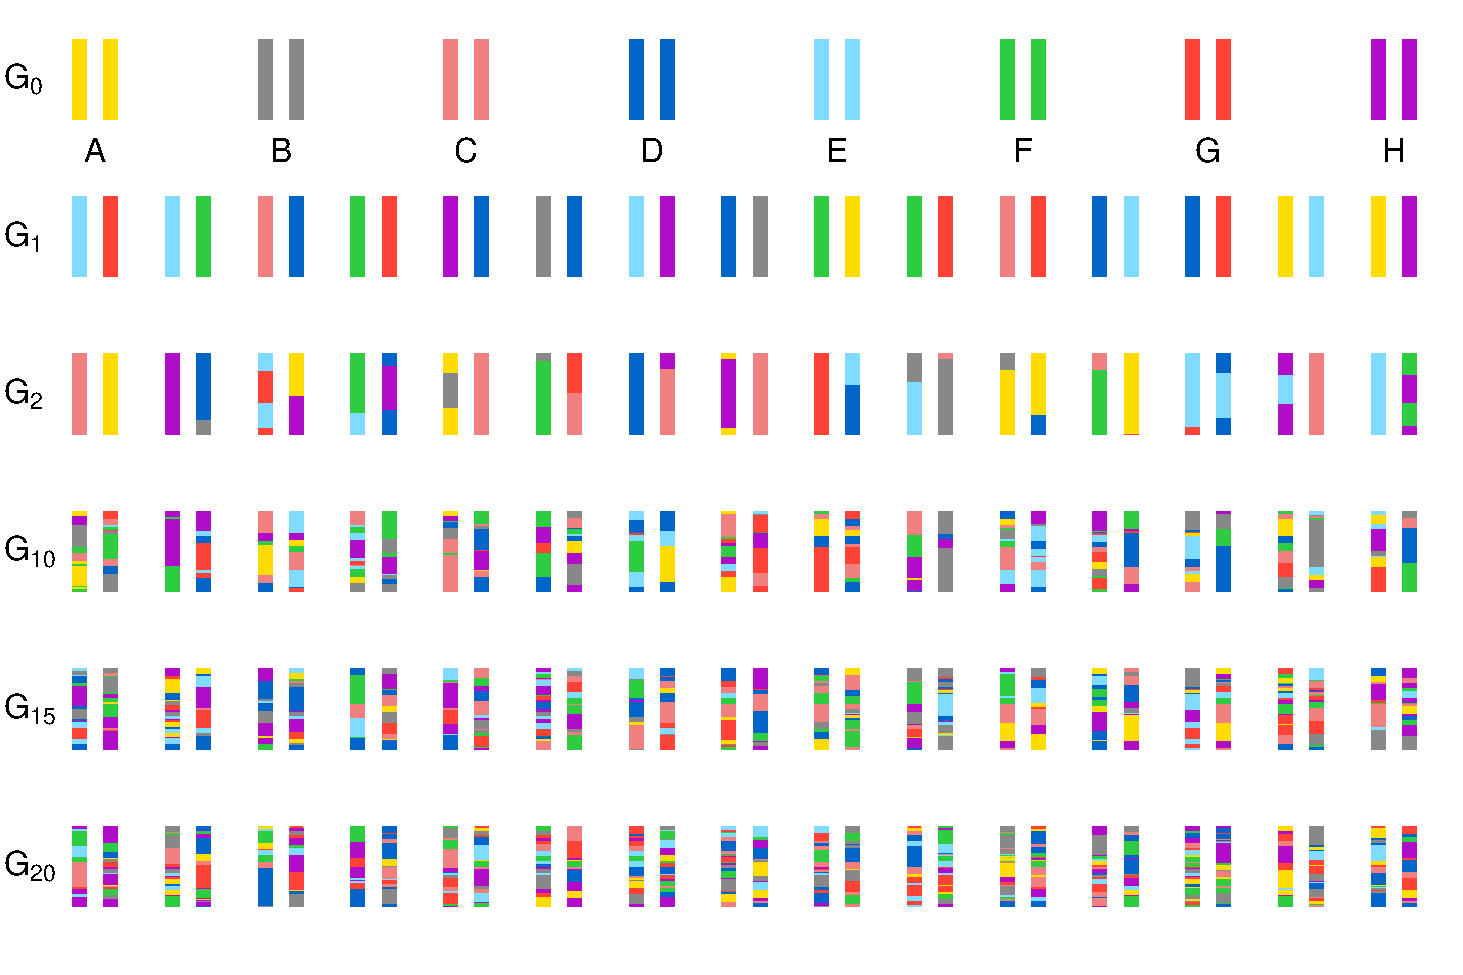
\includegraphics[height=0.95\textheight]{Figs/hs_light.pdf}
}


\end{frame}



\begin{frame}{The work}

    \bbi
  \item Collaboration
  \item Data exploration
  \item Methods development
  \item Software development
    \onslide<2>{
      \bi
    \item R
    \item C++
    \item Coffeescript
    \item Ruby
      \ei
    }
    \ei

\end{frame}



\begin{frame}{Qiongshi Lu}

\hspace*{0.85\textwidth}
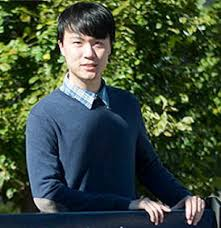
\includegraphics[height=1in]{Pics/qiongshi_lu.jpg}
\vspace*{-30mm}

{\large Human genome-wide association studies}

\bigskip

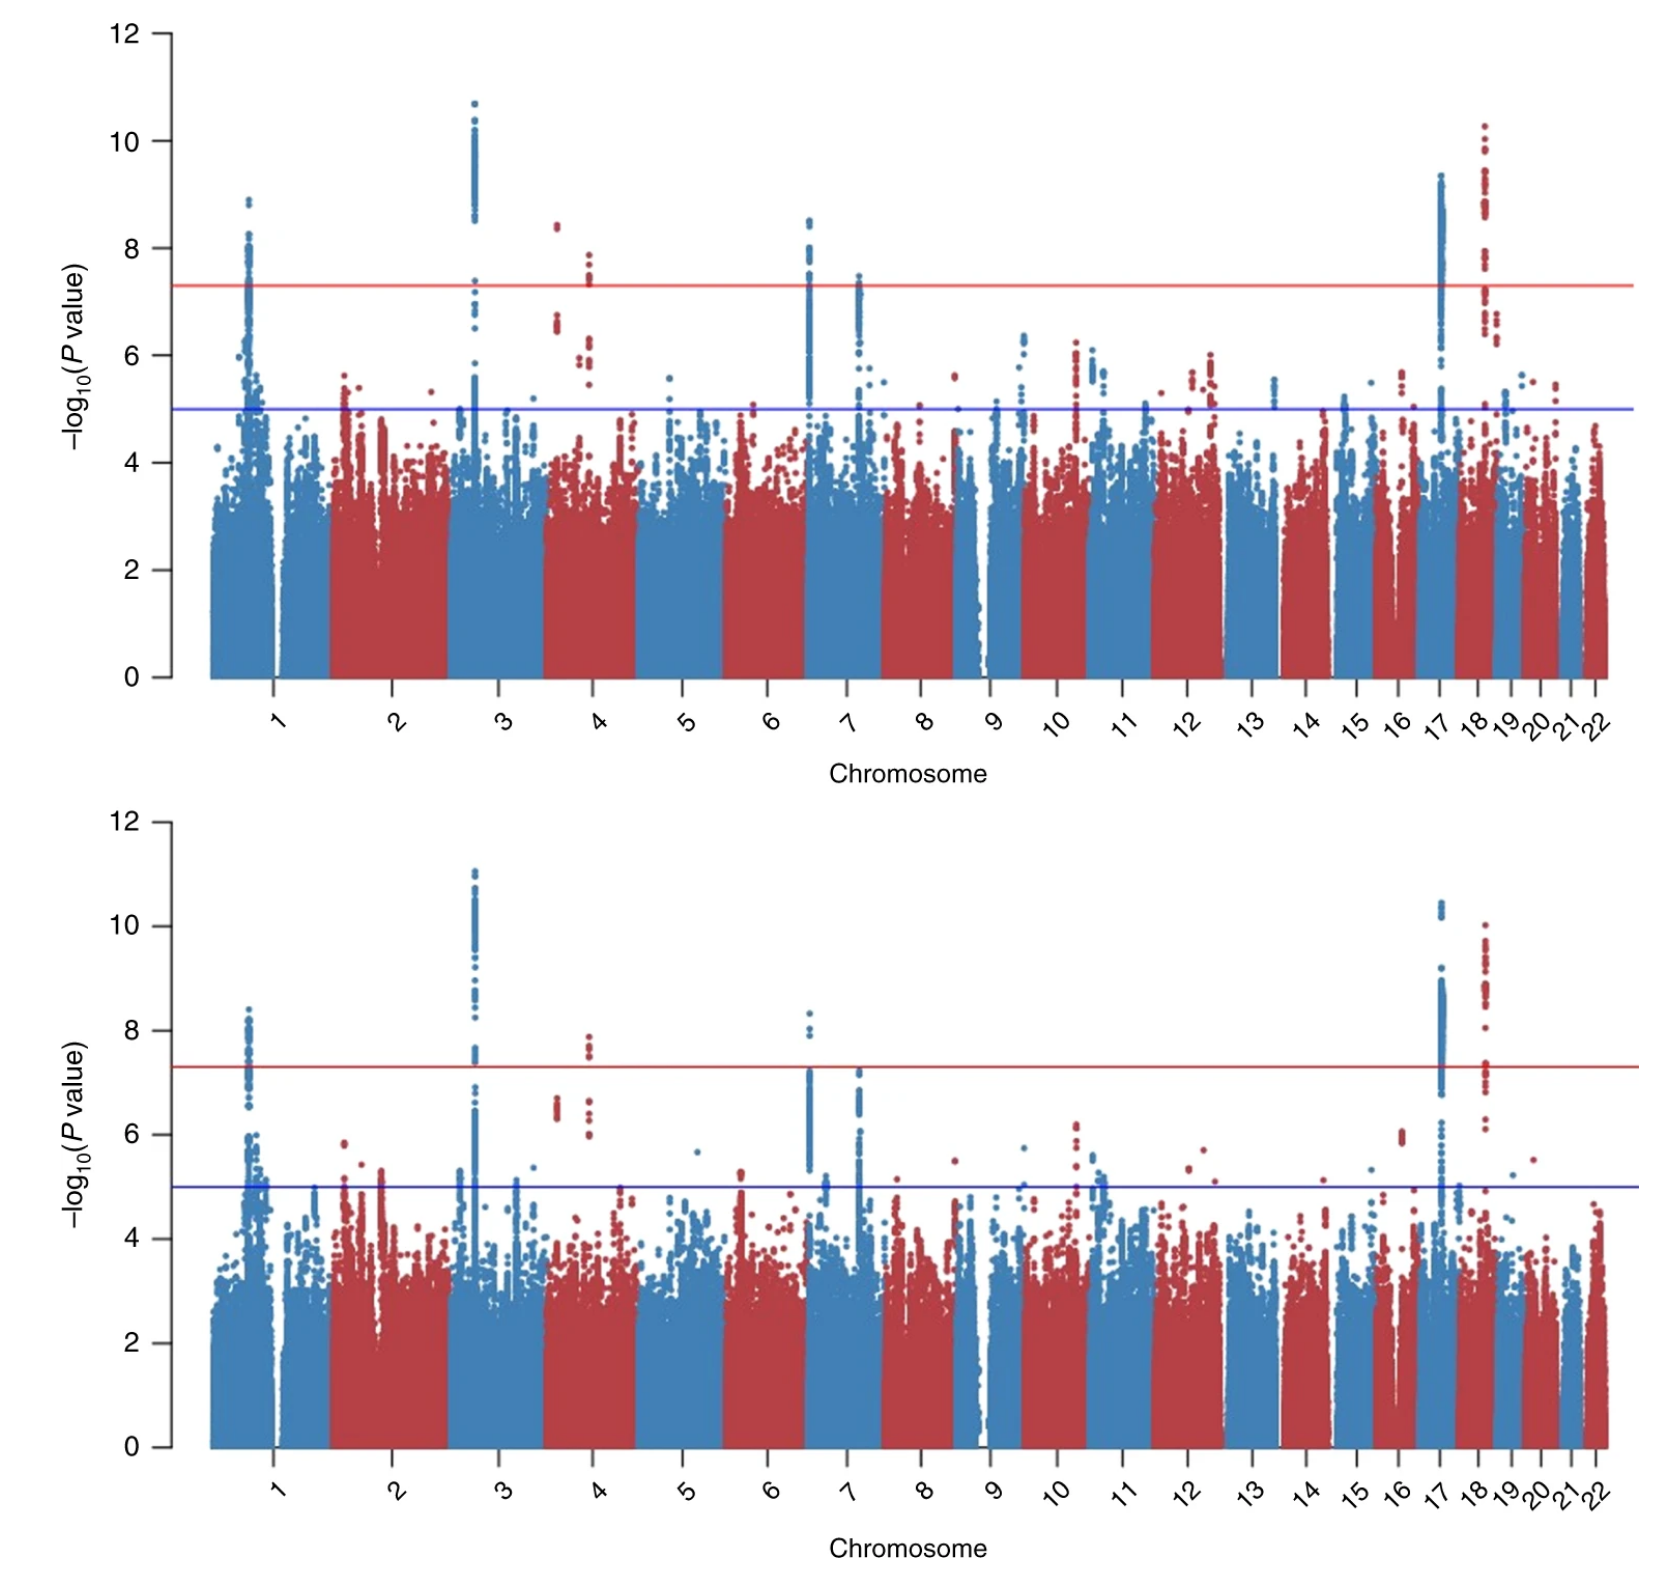
\includegraphics[height=68mm]{Pics/qiongshi_lu_gwas.png}


\end{frame}






\begin{frame}{S\"und\"uz Kele\c{s}}

\hspace*{0.85\textwidth}
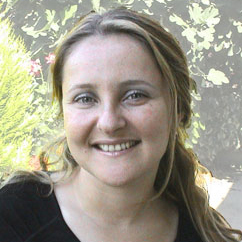
\includegraphics[height=1in]{Pics/keles.jpg}
\vspace*{-30mm}

{\large Functional mediation analysis}

\bigskip

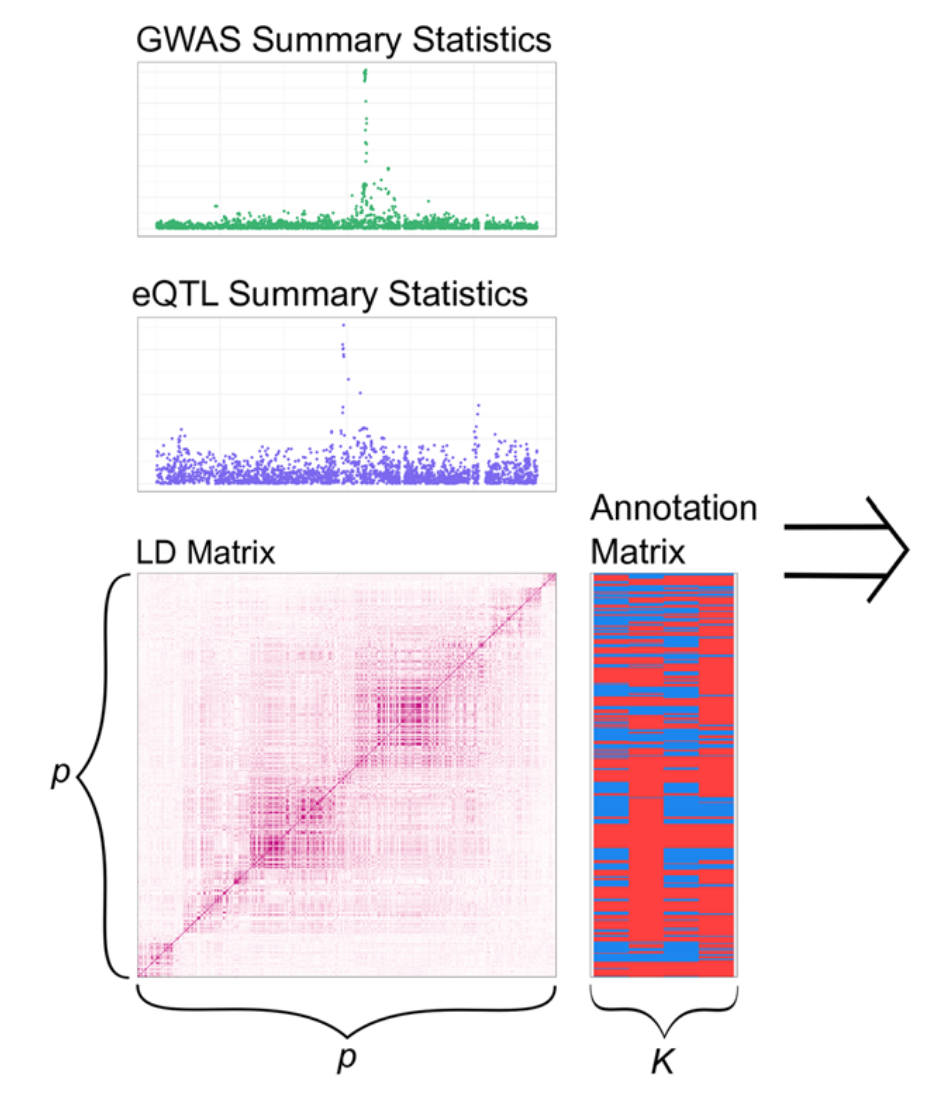
\includegraphics[height=68mm]{Pics/keles_mediation_A.png}
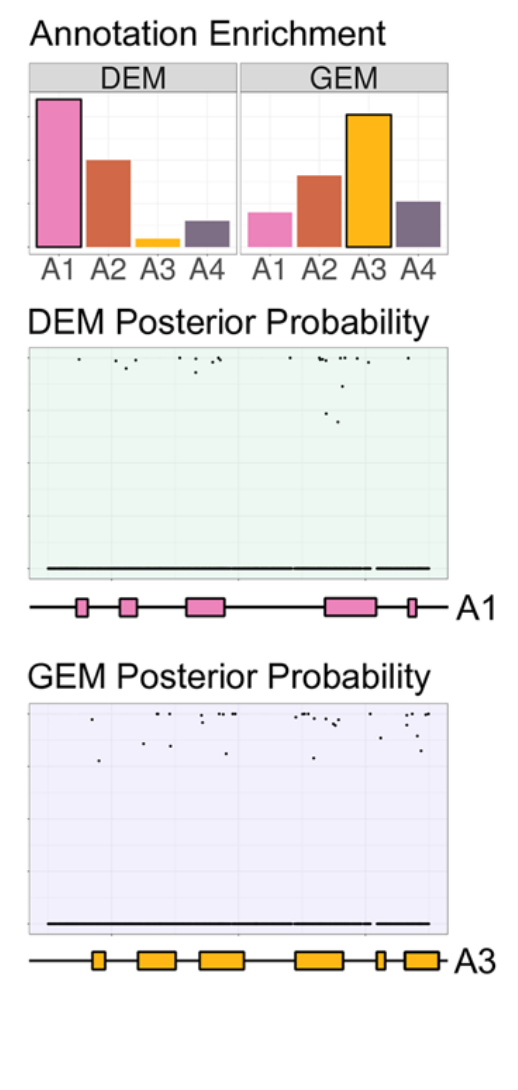
\includegraphics[height=68mm]{Pics/keles_mediation_B.png}


\end{frame}


\begin{frame}{Christina Kendziorski}

\hspace*{0.85\textwidth}
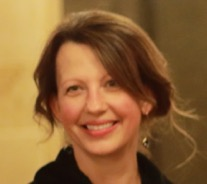
\includegraphics[height=1in]{Pics/kendziorski.jpg}
\vspace*{-30mm}

{\large Clock genes in stem cells}

\bigskip

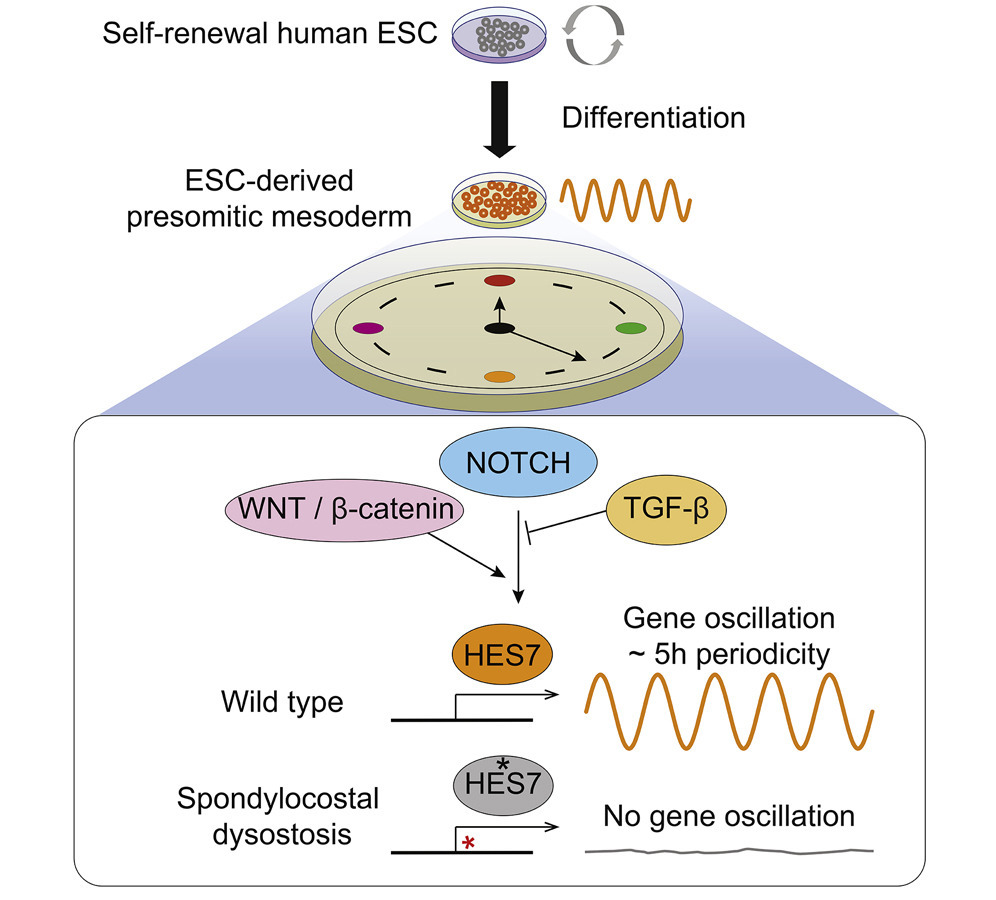
\includegraphics[height=68mm]{Pics/kendziorski_cellclock.jpg}


\end{frame}



\begin{frame}{Tony Gitter}

\hspace*{0.85\textwidth}
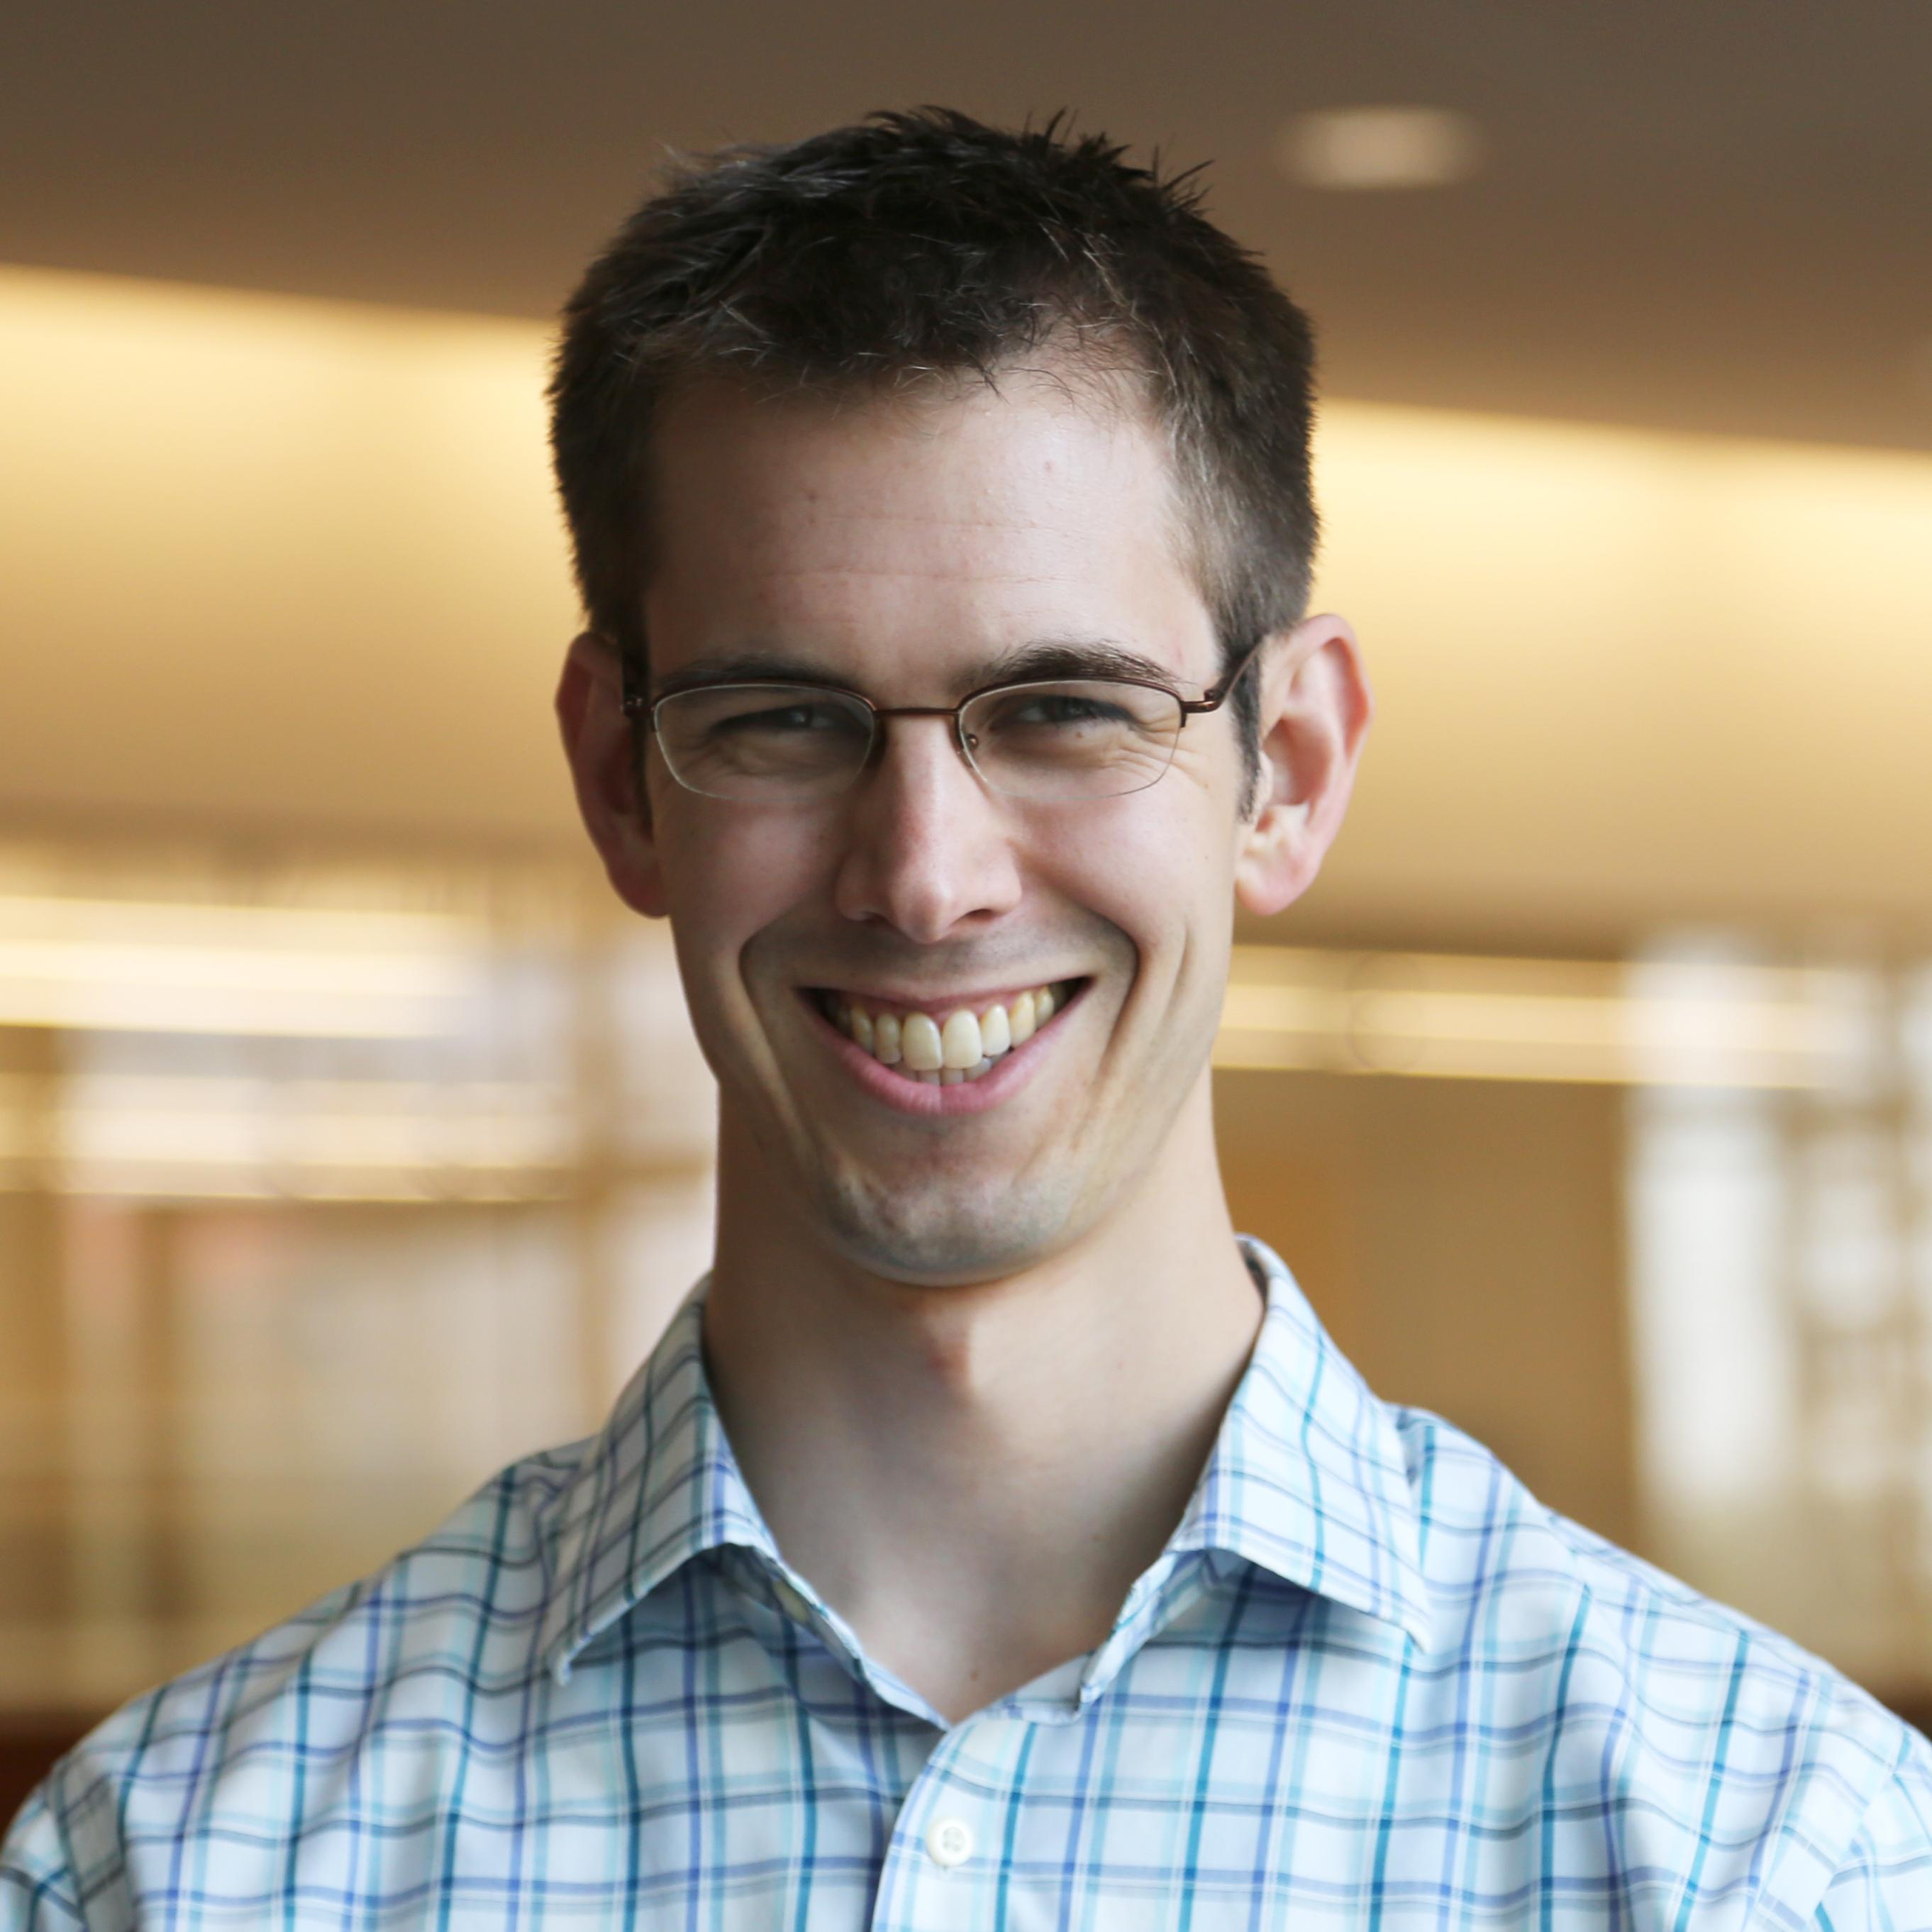
\includegraphics[height=1in]{Pics/tony_gitter.jpg}
\vspace*{-30mm}

{\large Pathways disrupted by cancer}

\bigskip

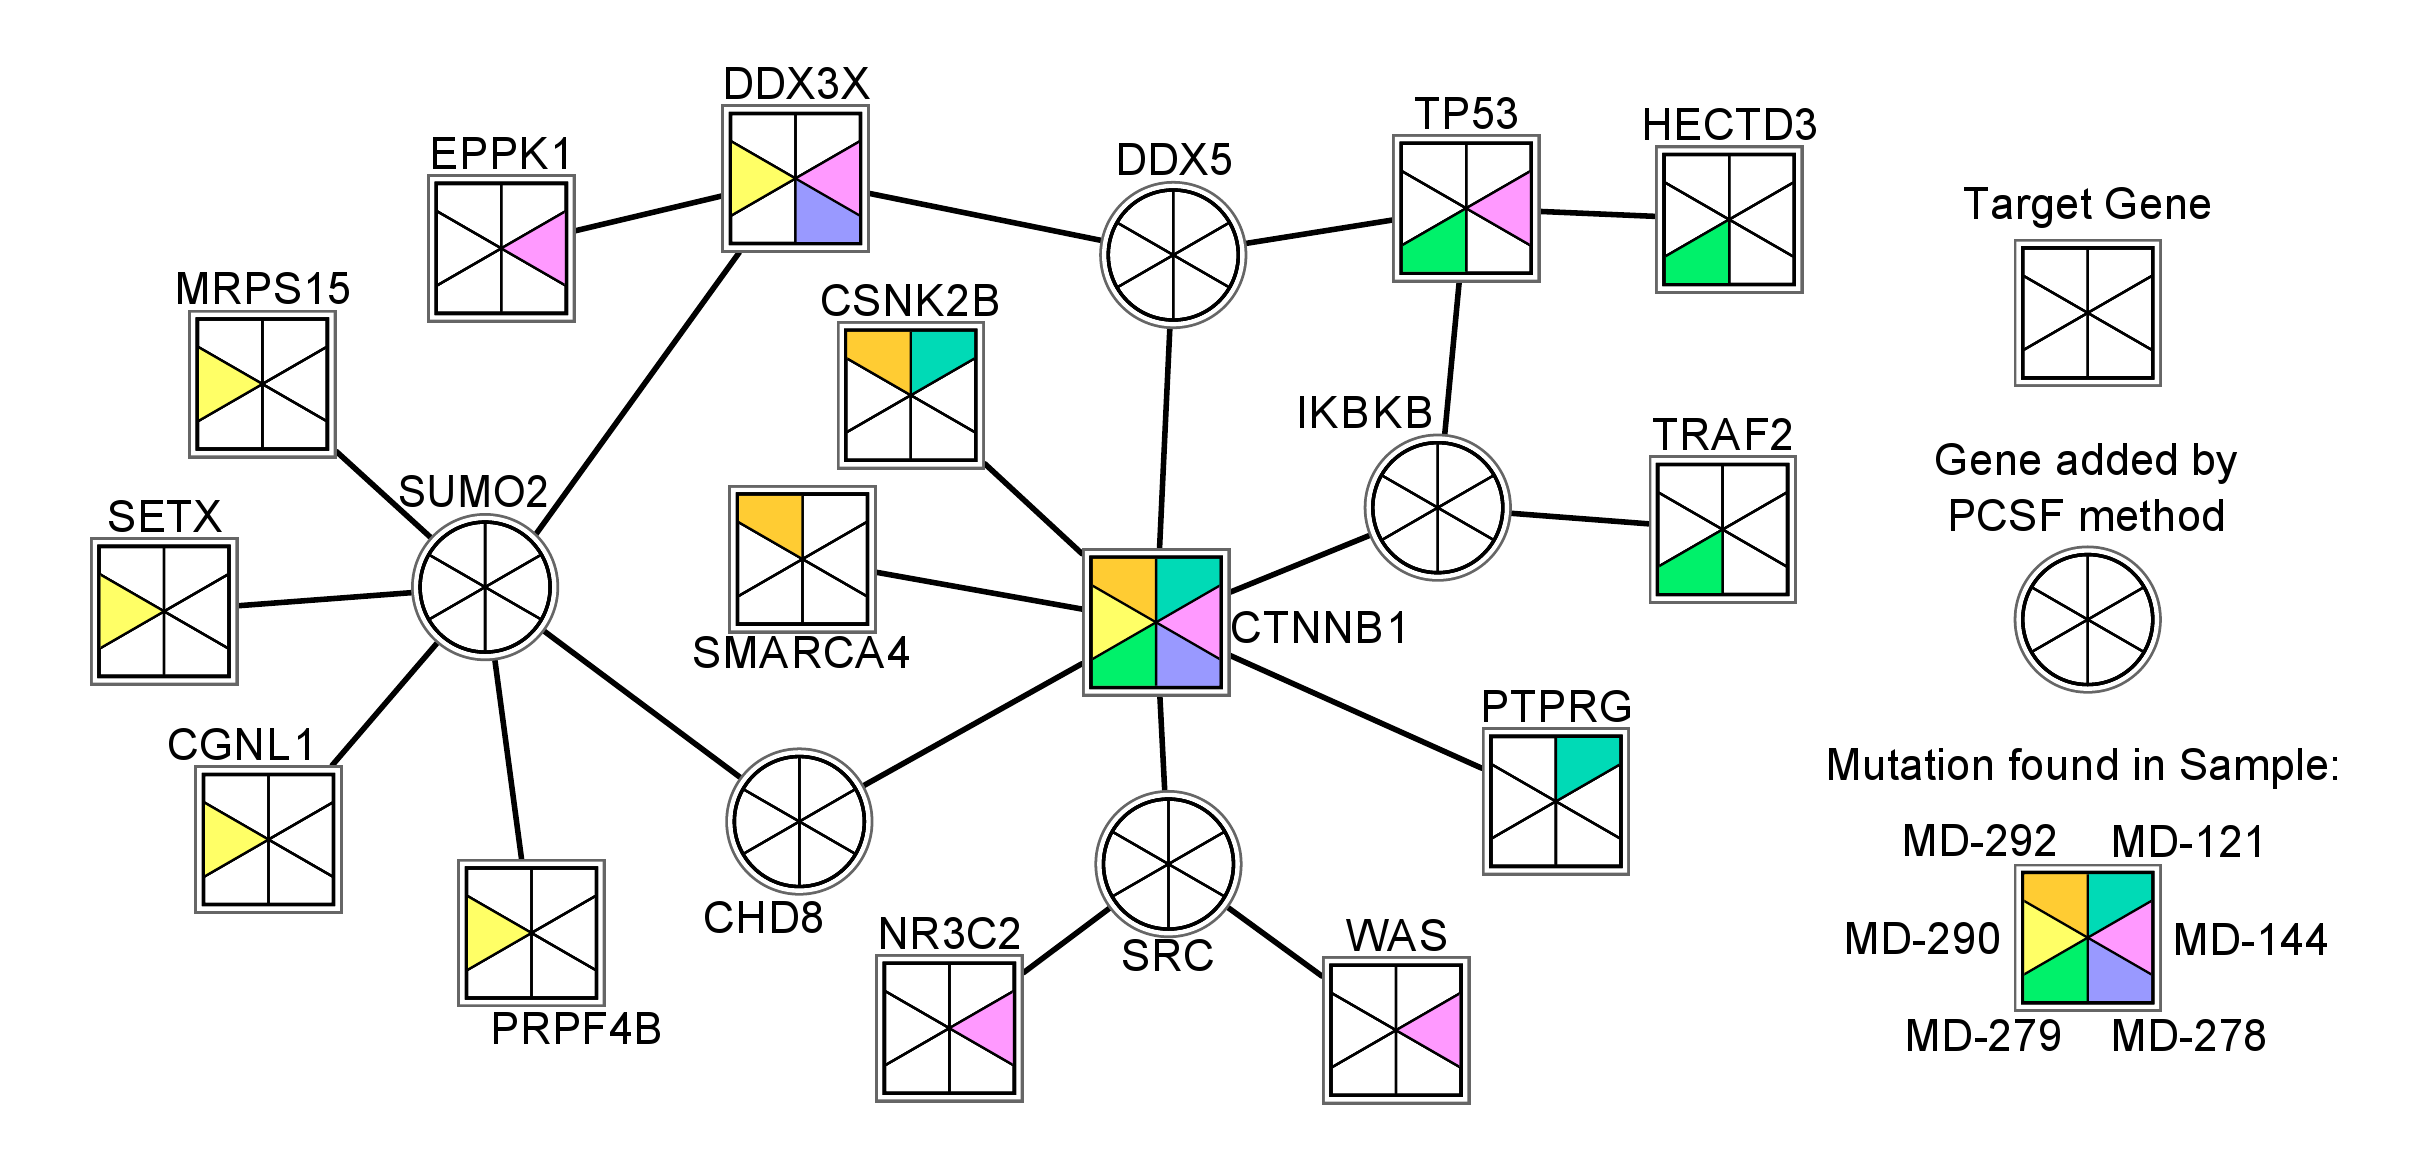
\includegraphics[height=55mm]{Pics/tony_gitter_MultiPCSF.png}


\end{frame}


\begin{frame}{Vikas Singh}

\hspace*{0.85\textwidth}
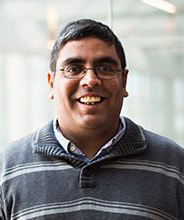
\includegraphics[height=1in]{Pics/vikas_singh.jpg}
\vspace*{-30mm}

{\large Analysis of brain images}

\bigskip

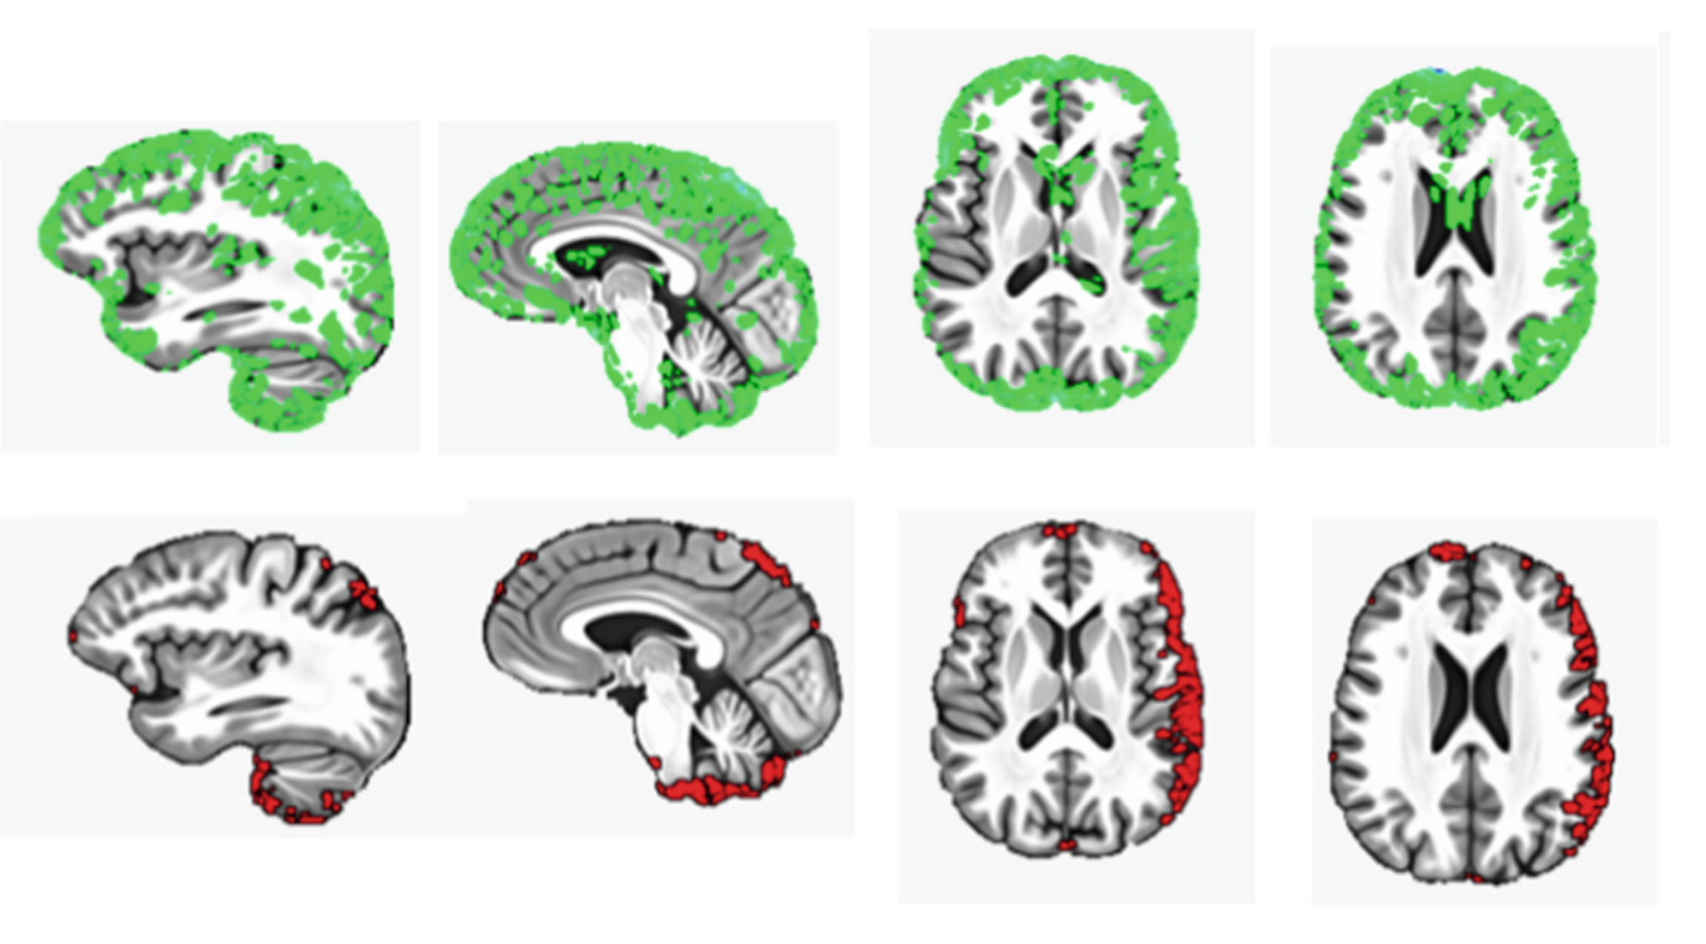
\includegraphics[height=64mm]{Pics/vikas_brains.png}


\end{frame}



\begin{frame}{Biomedical data science PhD at UW-Madison}

    \bbi
  \item Faculty spanning biostatistics, bioinformatics, and computer
    science
  \item Broad opportunities for scientific collaborations
  \item Flexible course requirements
  \item Research rotations
  \item Literature and professional skills seminars
    \ei


\bigskip \bigskip

\centerline{\href{https://bit.ly/MadBDS}{\Large \tt bit.ly/MadBDS}}

\end{frame}


\begin{frame}[c]{}

  \vspace{-10mm} \hspace*{-13mm}
  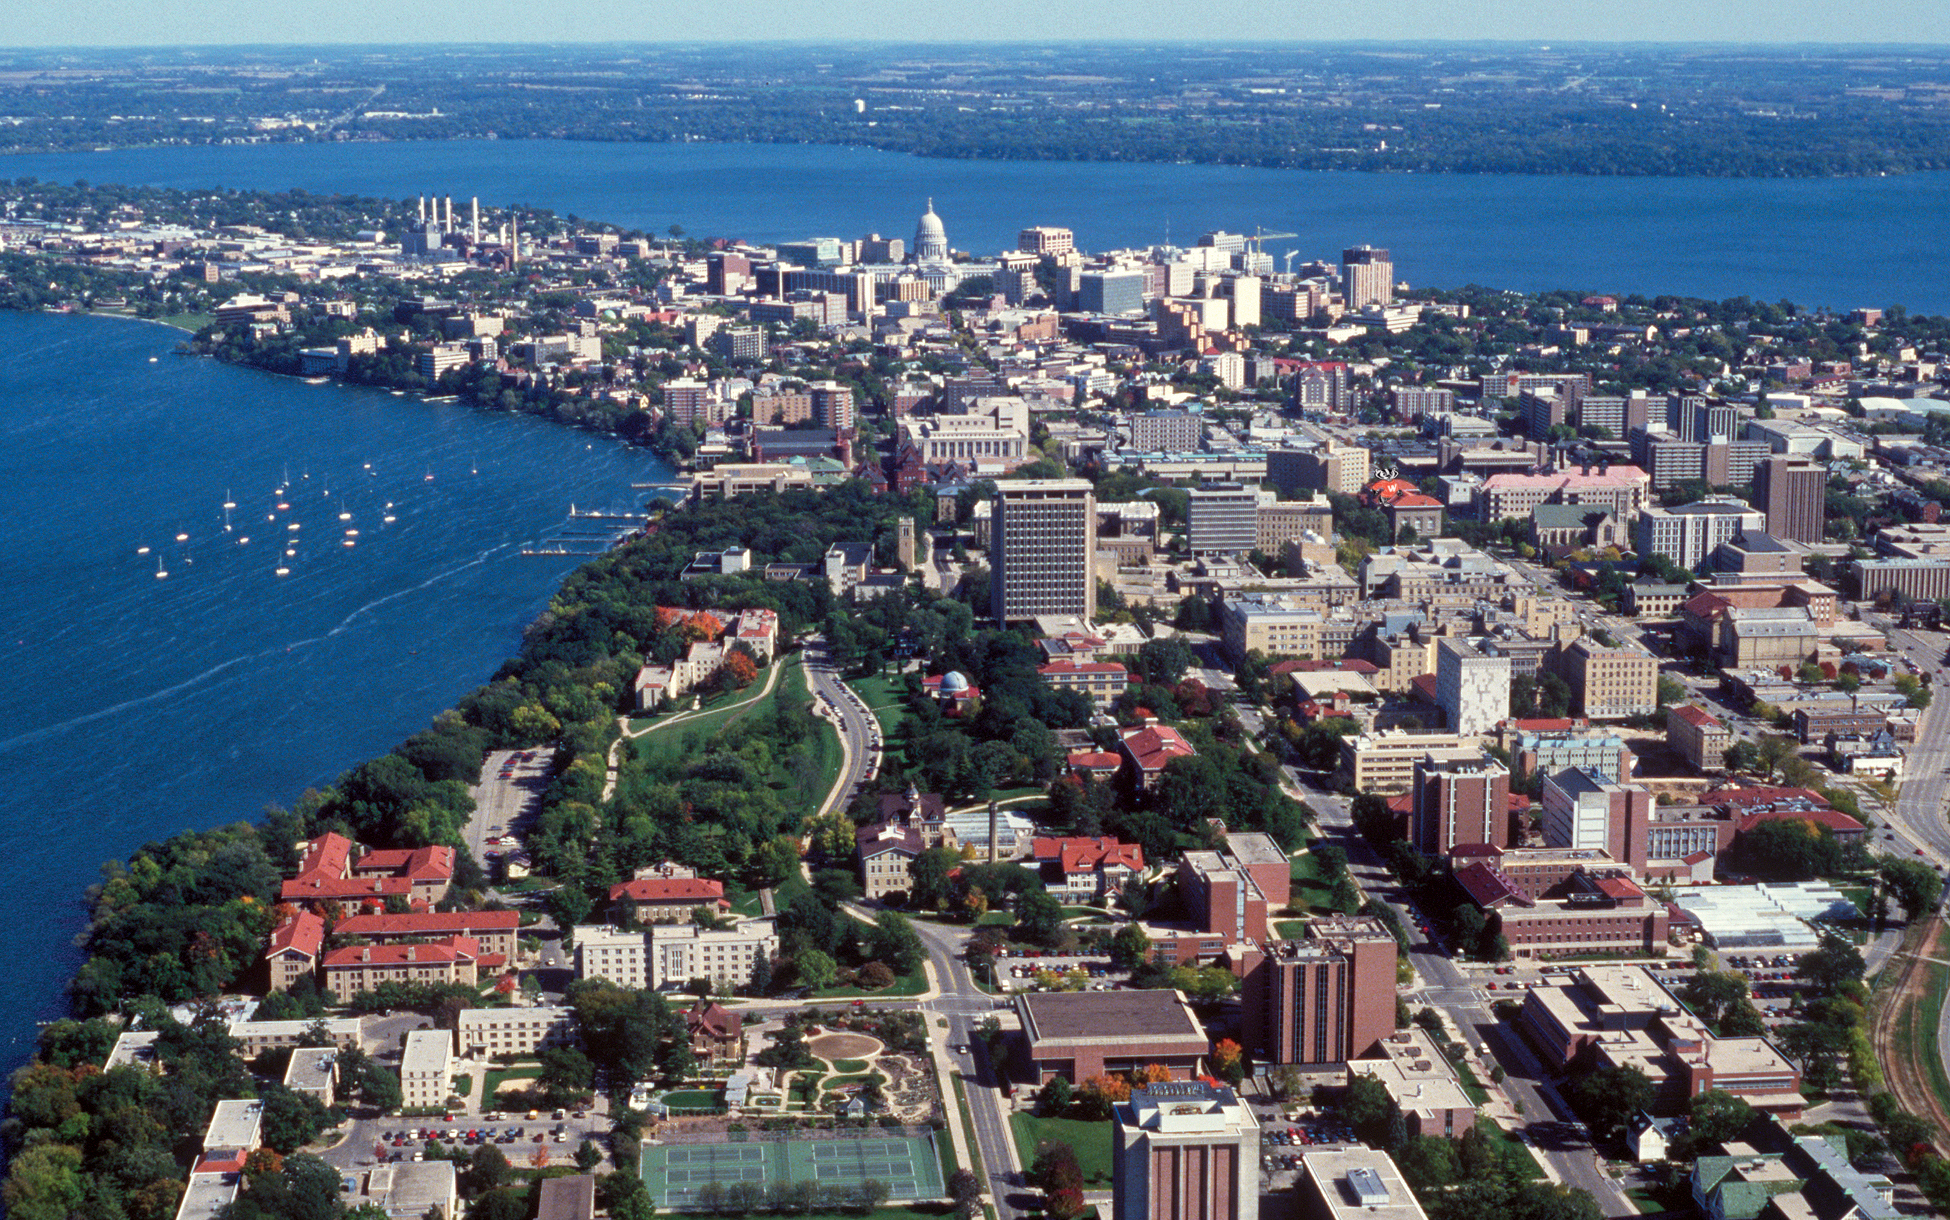
\includegraphics[height=1.2\textheight]{Pics/madison.jpg}

\end{frame}



\begin{frame}[c]{}

\Large

Slides: \href{https://bit.ly/carleton2019}{\tt bit.ly/carleton2019}

\vspace{7mm}

\href{https://kbroman.org}{\tt \lolit kbroman.org}

\vspace{7mm}

\href{https://github.com/kbroman}{\tt \lolit github.com/kbroman}

\vspace{7mm}

\href{https://twitter.com/kwbroman}{\tt \lolit @kwbroman}


\end{frame}

\end{document}
